\documentclass{beamer}

\mode<presentation>
{
  \usetheme{default}      % or try Darmstadt, Madrid, Warsaw, ...
  \usecolortheme{default} % or try albatross, beaver, crane, ...
  \usefonttheme{default}  % or try serif, structurebold, ...
  \setbeamertemplate{navigation symbols}{}
  \setbeamertemplate{footline}[frame number]
  \setbeamertemplate{caption}[numbered]
} 

\usepackage[english]{babel}
\usepackage[utf8x]{inputenc}

\usepackage{graphicx}
\usepackage{subcaption}
\usepackage{hyperref}
\usepackage{verbatim}

\title[Git for Economists]{Git and GitHub: A Guide for Economists}
\author{Frank Pinter}
\date{22 February 2019}

\AtBeginSection[]
{
  \begin{frame}
    \frametitle{Table of Contents}
    \tableofcontents[currentsection]
  \end{frame}
}

\begin{document}

\begin{frame}
  \titlepage
\end{frame}

\begin{frame}{Outline}
  \tableofcontents
\end{frame}

\section*{Introduction}

\begin{frame}{What is version control?}
Version control is a way to keep track of changes to code, text, and documents. And data and outputs.
\begin{itemize}
\item It gives you an organized revision history
\item It lets you experiment without fear
\item It lets you go back and forth between many different versions of the same file, and see a list of the differences
\item It makes (the technical aspects of) collaboration a breeze
\item It lets you and your collaborators work on different versions and then merge them
\end{itemize}
\end{frame}

\begin{frame}{What is Git?}
\begin{itemize}
\item Git is a program that does version control
\item It is the most popular version control program in software development
\item It is easy to set up and get started
\item There are many programs that add intuitive interfaces on top of Git
\item Git integrates seamlessly with online collaboration tools like GitHub and GitLab
\end{itemize}
\end{frame}

\section{The importance of version control}

\begin{frame}{Using it yourself}
Git isn't just useful for collaboration. It also helps you keep your own projects organized.
\end{frame}

\begin{frame}{Life without version control}
You're writing a paper and you have a regression.
\begin{itemize}
\item Advisor 1 tells you to include a certain variable. You put in lots of work to get the data, clean it, merge it, change the specification, and re-run.
\item Advisor 2 tells you that variable is dumb. You remove it.
\item Then Advisor 2 changes their mind.
\end{itemize}
What do you do?
\end{frame}

\begin{frame}{Life without version control}
Do you keep every specification you ever tried?
\begin{itemize}
\item The code and the outputs?
\item What if you discover a coding error that affects many of your specifications?
\item How do you organize all the files?
\end{itemize}
\end{frame}

\begin{frame}{Version control 0.1: putting dates on things}
Does this look familiar?
\texttt{run\_regs\_11\_17\_2018\_v4\_final\_final.do}
\\
``Not one piece of commercial software you have on your PC, your phone, your tablet,
your car, or any other modern computing device was written with the `date and initial' method.'' (Gentzkow and Shapiro)
\end{frame}

\begin{frame}{Version control 0.2: Dropbox}
\begin{itemize}
\item Dropbox keeps a crude version history.
\begin{itemize}
\item But there are no labels or comments, and it's not easy to see the differences between files.
\item So if you want to dig up ``the version where I had that other variable'' you have to manually look through a bunch of versions.
\item And good luck if you changed two scripts, not just one.
\end{itemize}
\item Dropbox lets you and your collaborators stay in sync.
\begin{itemize}
\item What if you and your coauthor try to change the same script at the same time?
\item What if you are trying one change and, at the same time, your coauthor is trying a different change?
\end{itemize}
\end{itemize}
\end{frame}

\begin{frame}{Version control 0.2: Dropbox}
A Post It note spotted on a grad student's desk:
\begin{quote}
	Don't forget! At 10:18 am on November 17th, we changed the specification to add new variable.
\end{quote}
Don't live this way.
\end{frame}

\section{Using version control}

\begin{frame}{Why use Git?}
Git is the dominant version control system today. There are others, but they're generally more work with no benefit.
\end{frame}

\begin{frame}{Getting started}
\begin{enumerate}
\item \href{https://git-scm.com/book/en/v2/Getting-Started-Installing-Git}{Install Git} (Linux, Mac, Windows)
\item Git comes with a command line interface (powerful!). You might want to add a graphical interface to make things easier:
\begin{itemize}
\item \href{https://www.gitkraken.com/}{GitKraken}
\begin{itemize}
\item The screenshots in this presentation are from GitKraken
\end{itemize}
\item \href{https://desktop.github.com/}{GitHub Desktop}
\item \href{https://support.rstudio.com/hc/en-us/articles/200532077-Version-Control-with-Git-and-SVN}{RStudio (for R projects)}
\end{itemize}
\end{enumerate}

\end{frame}

\begin{frame}{The Git model}

\begin{enumerate}
\item You do work in your \textbf{working directory}.
\item Then you add it to your \textbf{staging area}.
\item Once you've staged all your changes for one discrete task, \textbf{commit} a snapshot of the staging area.
\item If you have a remote repository, \textbf{push} your commit to the remote repository.
\end{enumerate}

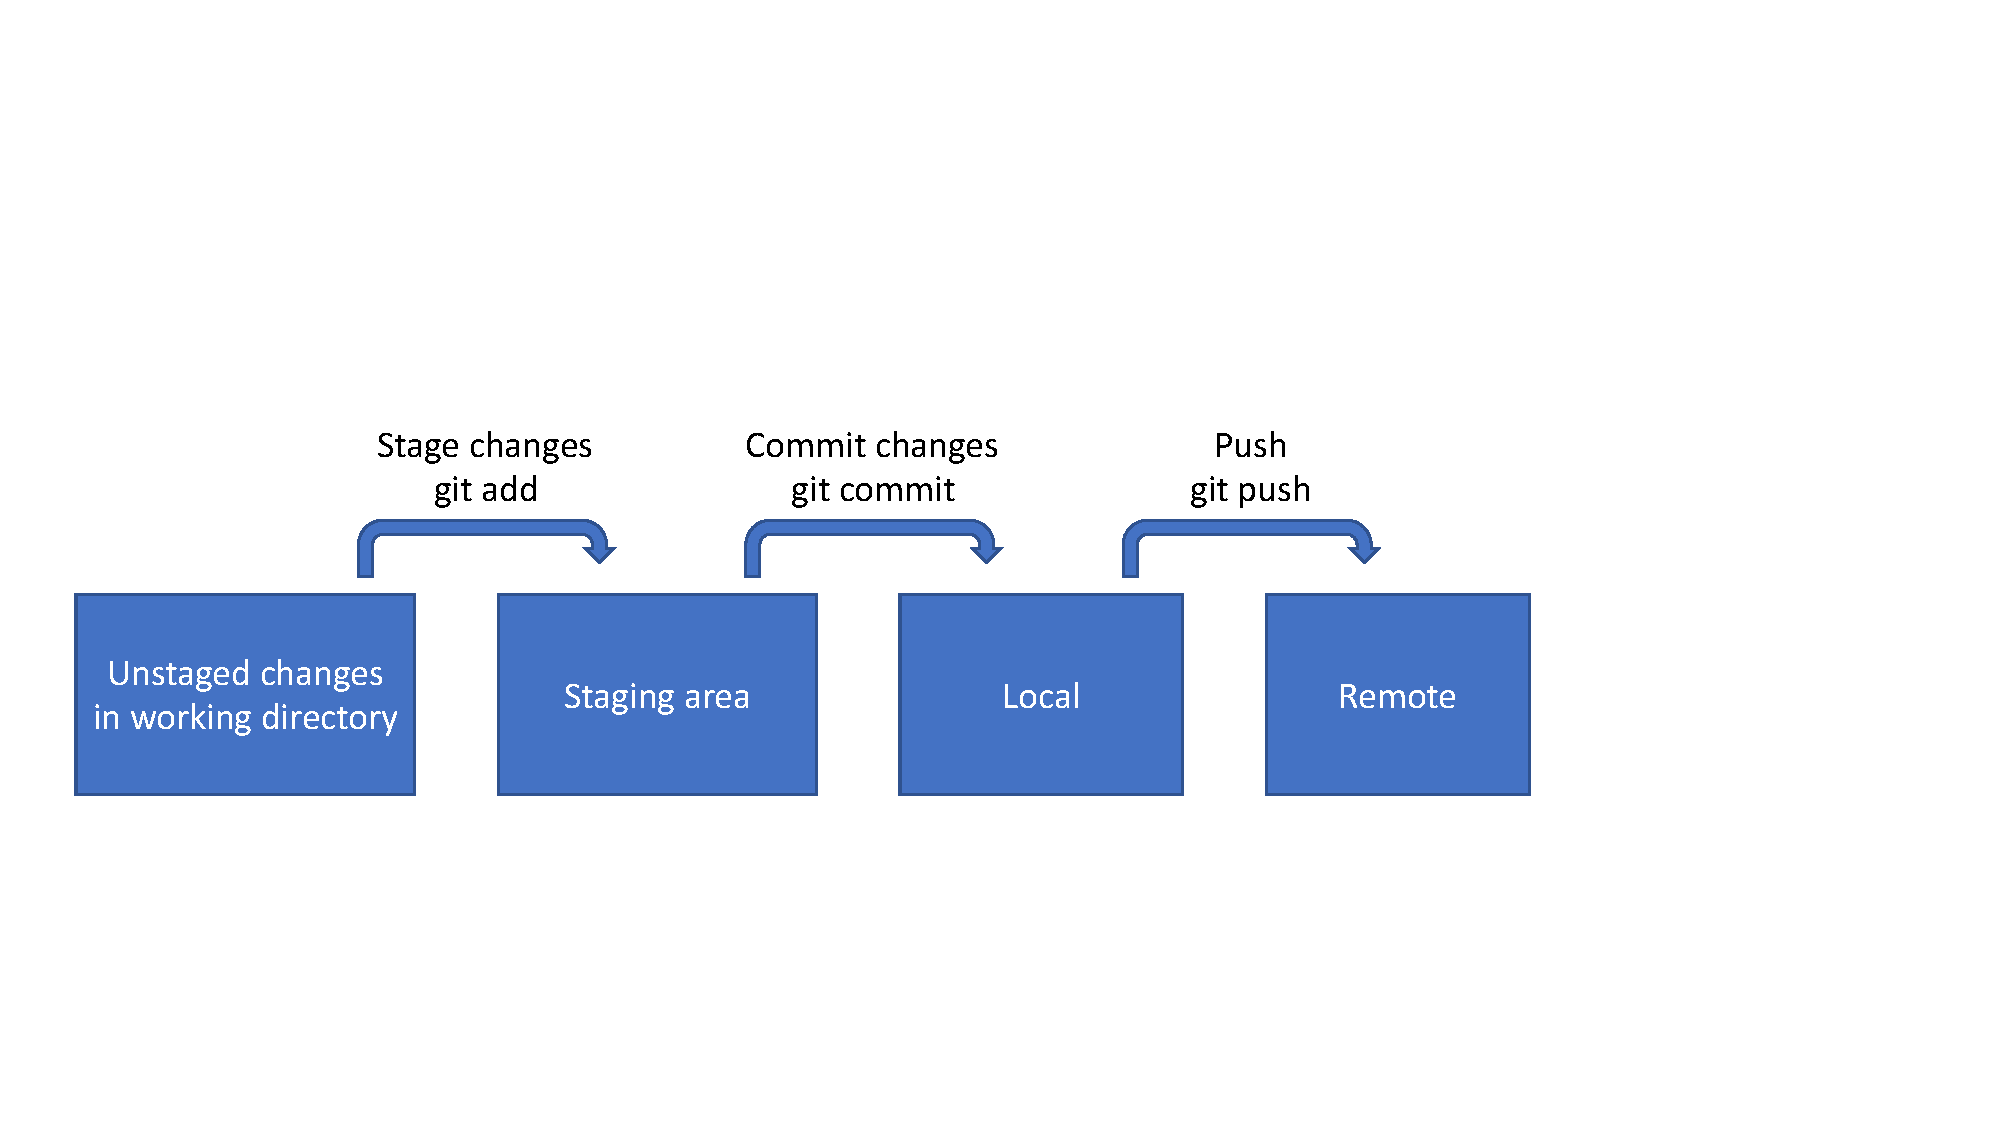
\includegraphics[width=\textwidth]{git-model.pdf}
\end{frame}


\begin{frame}{Commits: saving a snapshot}
What is ``one discrete task''? A collection of changes, across multiple files, that does \textit{one thing}. Examples:
\begin{itemize}
\item Change the formatting of a variable from string to numeric, and treat it properly across multiple scripts
\item Change your regression specification in code, in the output, and in your paper and supporting documentation
\item Add a new function, and tests for that function
\end{itemize}
These form one \textbf{commit}, which you annotate with a detailed \textbf{commit message}. Examples:
\begin{itemize}
\item ``Change the formatting of start date variable from string to Stata date format''
\item ``Add year dummies to regression specification''
\end{itemize}
The more detail, the more your future self will thank you.
\end{frame}

\begin{frame}{Commits}
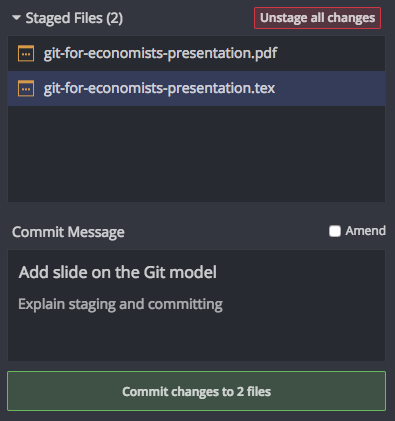
\includegraphics[width=200px]{screenshots/committing.png}
\end{frame}

\begin{frame}{Run tests before you commit}
Your code should run properly when you commit.
\begin{itemize}
\item No runtime errors
\begin{itemize}
\item Test this by running all code that changed, and everything that depends on it
\item Makefiles automate this process
\item Only skip if you are sure you didn't change anything important
\end{itemize}
\item No compilation errors (including \LaTeX)
\item Tests should pass
\item Output should be consistent with what you've written
\begin{itemize}
\item Don't report a negative regression coefficient, and write in words that the estimated coefficient is positive
\end{itemize}
\end{itemize}
But it's better to have frequent commits (that might have small mistakes) than to have giant, infrequent commits.

{\tiny You can also do partial commits (\texttt{git add --patch}) which are somewhat advanced.}
\end{frame}

\begin{frame}{What should I include?}
\begin{enumerate}
\item At a minimum:
\begin{itemize}
\item Code (\texttt{.do}, \texttt{.R}, \texttt{.m}, \texttt{.jl}, and so on)
\item Text files (\texttt{.txt})
\item \LaTeX \, documents (\texttt{.tex})
\end{itemize}
\item I also recommend:
\begin{itemize}
\item Raw \texttt{.csv} datasets, if small (\textless 10 MB)
\end{itemize}
\item These are binary files, so you can't see differences between versions. I recommend including them anyway.
\begin{itemize}
\item PDF files
\item Word, Excel, PowerPoint files
\end{itemize}
\item Some people also include all datasets.
\begin{itemize}
\item Note that GitHub doesn't allow files larger than 100 MB, or projects with total size larger than 1 GB.
\end{itemize}
\end{enumerate}

For datasets, look into \href{https://git-lfs.github.com/}{Git Large File Storage}.
\end{frame}

\begin{frame}[fragile]{What should I exclude?}
In order to avoid driving your coauthors crazy, you \textbf{must} tell Git to ignore the junk files using a file called \textit{.gitignore}. It looks like this:

\begin{verbatim}
# Junk created by LaTeX
*.synctex.gz
*.out
*.log
# Junk created by R
.RData
# Junk created by Python
*.pyc
\end{verbatim}

Best practice: use \textit{.gitignore} to explicitly exclude \textit{everything} that you don't want to include, and commit \textit{.gitignore} like any other regular file.

GitHub maintains a \href{https://help.github.com/articles/ignoring-files/}{list of standard \textit{.gitignore}} files for many common languages.
\end{frame}

\begin{frame}{Viewing changes: diff}
Git easily lets you see what changed in \LaTeX, code (not images/PDFs/most datasets). Review this when staging!
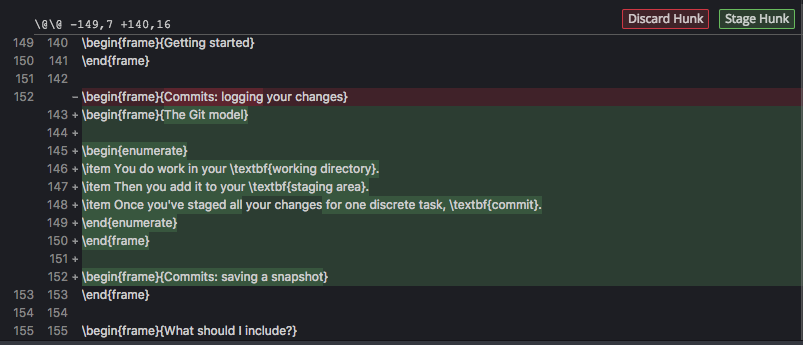
\includegraphics[width=\textwidth]{screenshots/diff.png}
{\small (This is the GitKraken interface, but it looks similar in any other interface)}
\end{frame}

\begin{frame}{Viewing changes: diff}
You can also go back and see past changes.
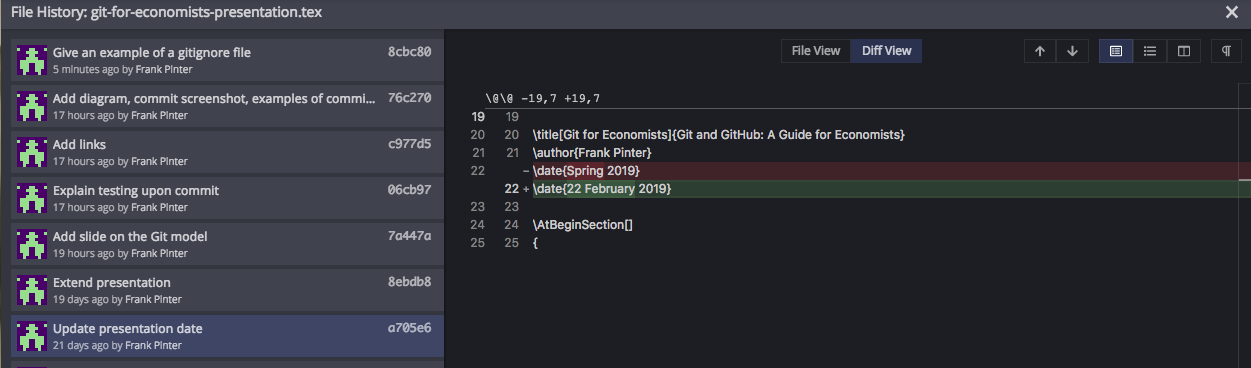
\includegraphics[width=\textwidth]{screenshots/history-diff.png}
\end{frame}

\begin{frame}{Branches: trying things out}
\href{https://git-scm.com/book/en/v2/Git-Branching-Branches-in-a-Nutshell}{Branches} are the most powerful part of Git
\begin{itemize}
\item By default, all the work you do goes into the ``master'' branch
\item Want to experiment? Start a new branch
\item You can switch between branches, and make commits to either branch
\begin{itemize}
\item There is a catch: if you don't include your intermediate/final datasets in Git, you may need to re-make them when you switch
\end{itemize}
\item If your experiment works out, commit and merge back into the master branch
\begin{itemize}
\item If there are conflicts between the commits you've made on the two branches, Git will ask you to resolve them
\item This is easiest with a graphical interface like \href{https://support.gitkraken.com/working-with-repositories/branching-and-merging/}{GitKraken}
\end{itemize}
\item If your experiment doesn't work out, delete the new branch painlessly
\item The best way to learn how to use branches: practice
\end{itemize}
\end{frame}

\begin{frame}{Keeping it local vs. using a remote repository}
Git doesn't require a remote repository. You can run it 100\% on your computer, with no connection to an outside server.
\begin{itemize}
\item This is useful if you have restrictions on your code (for example, you work with confidential health data)
\begin{itemize}
\item Ask me if you have questions about using Git this way on the NBER cluster
\end{itemize}
\item But a remote repository helps you keep things backed up seamlessly, and lets you collaborate with others
\item You can push all your branches to the remote repository, or only some of them
\end{itemize}

\end{frame}

\section{Using Git for collaboration}

\begin{frame}{Repos}
\end{frame}

\begin{frame}{What's GitHub?}
\end{frame}

\begin{frame}{Brief detour: hosting services}
\begin{itemize}
\item With a free GitHub account, you can create
\begin{itemize}
\item as many private repositories as you want
\item but each private repository can only have three collaborators.
\item You can also create as many public repositories as you want (and each can have as many collaborators as you want).
\end{itemize}
\item GitLab is a competing service. With a free GitLab account, you can create as many private repositories as you want, with as many collaborators as you want.
\item It's easy to use GitHub for one project, and GitLab for another
\end{itemize}

\end{frame}


\section*{Conclusion}

\begin{frame}{Conclusion}
\end{frame}

\begin{frame}{Further reading}
\begin{itemize}
\item Matt Gentzkow and Jesse Shapiro, ``Code and Data for the Social Sciences: A Practitioner’s Guide'' (\url{https://web.stanford.edu/~gentzkow/research/CodeAndData.pdf}). See Chapter 3 for more on why you should use version control.
\item Jes\'us Fern\'andez-Villaverde's notes on high-performance computing (see also his class Computational Economics). Chapter 5 (\url{https://www.sas.upenn.edu/~jesusfv/Chapter_HPC_5_Git.pdf}) is an extended Git tutorial using the command line interface.
\item Hadley Wickham's book on writing R packages. The chapter on Git and GitHub (\url{http://r-pkgs.had.co.nz/git.html}) is well-written and not specific to R.
\end{itemize}
\end{frame}

\end{document}
